\section{Design}

\subsection{Architecture}

\begin{figure}[!h]
\centering
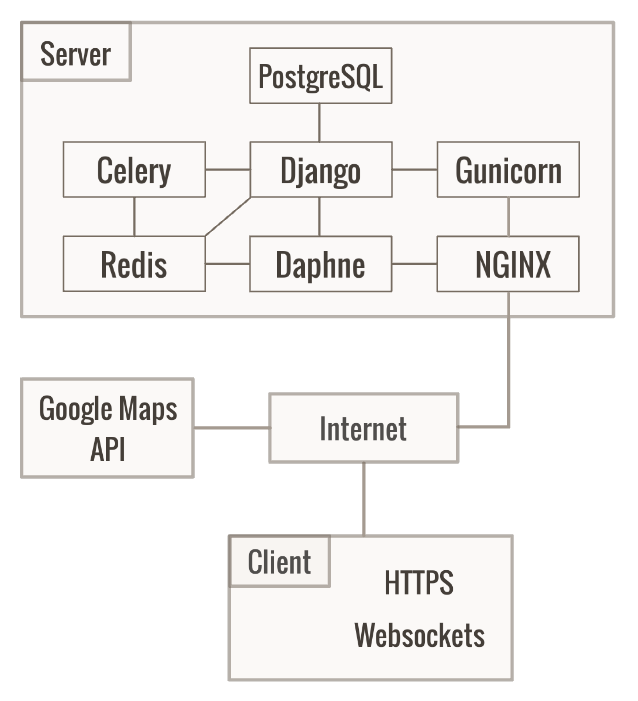
\includegraphics[width=250px]{assets/architecture.png}
\caption{Architecture map for \emph{localhost}}
\label{fig:architecture_map}
\end{figure}

\subsubsection{Execution Path}

When navigating to \emph{localhost}, the client is connected to the NGINX
service. If the required page is a static file such as a CSS or JavaScript
file then the file is immediately served by NGINX. WebSocket requests are
forwarded to the Daphne service (see Section \ref{realtime}). All remaining
requests are forwarded to the Gunicorn web server to then be redirected to
Django.

\subsubsection{Scalability}

The architecture behind \emph{localhost} was designed with scalability as a
priority. The core services on the server are Django and PostgreSQL.
Having multiple other services running concurrently reduces the computation
time available for the core services. While \emph{localhost} was deployed on
a single server, the architecture is designed so that services like NGINX can
be deployed on separate servers. As NGINX handles the majority of requests
across the web, moving NGINX to a separate server would significantly improve
the performance of the platform. Each non-core service can have multiple
workers and deployed on multiple servers, ensuring that \emph{localhost} is
scalable.

\subsection{User Interface}
Our vision for \emph{localhost} was for a simple, modern and user-friendly user
interface across all devices as current solutions, whilst flexible, allow hosts
to overload their listings which may cause them to lose potential tenants.

\subsubsection{Cross browser and mobile compatibility}

As we envisioned for \emph{localhost} to operate on desktop and mobile devices,
Bootstrap was deemed the most viable library to use as it is responsive and
designed mobile-first. The challenge we faced using Bootstrap was that the custom
templates for objects and designs were outdated and, while extremely functional
and simple to prototype, was more difficult to restyle to suit our modern theme.
This led us to discover Bootstrap Material, a fork of Bootstrap, which combined
the responsiveness of Bootstrap with a modern and appealing interface.

\subsubsection{Property Item Grouping}
On most preexisting platforms, multiple listings in the same property or building
would result in a separate search result returned for each listing. Our solution
to this was to have a \emph{Property} listing which would encapsulate all of the
individual listings as \emph{Property Items}. This is a major benefit as it
simplifies the listing process for hosts, requiring them to upload only one set
of pictures common to all the listings to the \emph{Propety}, and unique images
to each \emph{Property Item}, hence, less storage space will be utilised on the
server. Furthermore, this optimisation declutters the search results for
prospective tenants, allowing them to view a larger variety of properties.

\subsubsection{Information Limitation}
To combat the information bloat that exists on most current services, our system
enforces a word limit on both the description and title of each property and
property item. Instead, we encourage hosts to post pictures of their property and
select the amineties it has to offer which get reduced down to icons for
consistency and clarity.

\subsubsection{Google Maps API}
The Google Maps API was used for this project because of its powerful search
engine and its ability to scale with our architecture. The autocomplete on the
search bars are powered by this and when a user selects a location to base their
search on, the API breaks it down into the longitude and latitude values which
get utilised in the back-end of the platform. Maps on each property page are also
generated by the API.

\subsubsection{Modifications from User Testing}
We conducted a series of user tests, which can be viewed in the appendix, which
were evaluated and factored into future revisions of the design of the user
interface of \emph{localhost}. A few of these included certain features being
unclear or not obvious enough due to poorly coloured buttons or fonts, overly
strict requirements on account creation, unoptimised process flow for users when
performing certain actions such as not being able to message a host from their
listing pages, and many more.

\subsection{Database Design}

\subsubsection{Database of localhost}

An ER diagram of our database can be found in /docs/assets/models.jpg in our repository.
The database of \emph{localhost} is normalised in 3NF (third normal form) meaning it
contains no transitive dependencies, minimising our data redundancy and
improving data integrity. Extensibility was kept in mind when designing the
database. As an example, amenities have a many-to-many relation with property items
instead of being hard-coded into property items, meaning if our platform was to
support additional amenities, we can simply add those to our Amenities table rather
than changing our database structure.

\subsubsection{Property Search Time Optimisation}
One of the significant features in the application is searching for properties based on
their distance. A user can enter an address in the search bar and properties
near the search location will be displayed in the results page, sorted by
distance. There are several ways to implement the property search and we considered
three implementations:

\begin{enumerate}
  \item Use GeoDjango with PostGIS, and migrate our property model to use
    geometry field in GeoDjango.
  \item Store latitude and longitude for each property, then use an extension
    ``Geopy'' to approximate distances between properties in \texttt{QuerySet}
    and the search location~\parencite{geopy-doc}.
  \item Store latitude and longitude for each property, then annotate each item
    in \texttt{QuerySet} with built-in SQL function expressions to calculate the
    distance between search location and each property, then sort by that
    distance.
\end{enumerate}

Implementation 1 provides the most accurate distance approximations as GeoDjango supports
querying and manipulating spatial data in the database, which takes into account
elevations and sea level~\parencite{geodjango-raster-lookups}. However, the
accuracy gained from this framework is negligible when compared to the accuracies
of Implementations 2 and 3. Our final implementation was accurate to within 50m of the
target location, which is enough accuracy for sorting properties.
The effort to set up and migrate to a new database framework was thought to be
too much work for little gain.

Implementation 2 which calculates distances using Geopy was our second consideration.
Algorithm \ref{alg:geopy-search} roughly shows how we implemented the search and sorting
using GeoPy.

\begin{algorithm}
  \caption{Inefficient implementation of property search}\label{alg:geopy-search}
  \begin{algorithmic}
    \STATE $qs\gets Property.filter(critieria)$
    \STATE $lat, lng\gets urlparam.get(lat), urlparam.get(lng)$
    \STATE $properties\gets list()$
    \FORALL{$property$ in $qs$}
    \STATE $distance\gets geopy.distance((lat, lng), (property.lat, property.lng))$
    \STATE $properties.append(property, distance)$
    \ENDFOR
    \STATE $properties\gets sorted(properties, key=\lambda x: x[1])$
  \end{algorithmic}
\end{algorithm}

Algorithm \ref{alg:geopy-search} works well for small data sets
but the performance drops as the number of properties grows. Distances are
calculated using Python calls which could be far slower than SQL functions,
since most of the computations are done using GeoPy. For a large dataset of properties,
performance would be poor.

Having considered these alternatives, we chose to use Implementation 3 which uses
native SQL expressions to compute the distances which greatly improves
performance. To approximate distances using native SQL expressions, we need a
function/formula to translate latitudes and longitudes in the database model to
actual distances on the Earth.

\paragraph{Haversine Formula}\label{eq:haversine}
The haversine formula is used to determine the great-circle distance between two
points on a sphere given their longitudes and
latitudes~\parencite{haversine-formula}.
\[
  d = 2r\arcsin{\sqrt{\sin^2\left(\frac{\phi_2 - \phi_1}{2}\right) +
      \cos(\phi_1)\cos(\phi_2)\sin^2\left(\frac{\lambda_2 - \lambda_1}{2}\right)}}
\]
where,
\begin{itemize}
  \item $\phi_1, \phi_2$ are latitude of search location and latitude of property
  \item $\lambda_1, \lambda_2$ are longitude of search location and longitude of
    property.
  \item $r$ is the radius of the Earth
\end{itemize}

Our search query calculates the distance from each property to the target
destination using Haversine's Formula and then orders them by closest distance.

Since it is costly to calculate this for every property in the database, an
initial filter was added to narrow down the number of properties that the
distance calculation had to be operated on.
Only properties within $\pm$0.15 latitude and longitude offsets of the original
search, which translates to around 15km have their distance approximated using
Haversine's Formula. This greatly improves the
search times and also removes properties that are outside a reasonable distance
from the search. By adding the initial filter, our search time is also no longer
restricted by the property dataset and is instead limited by suburb density.

\begin{figure}[!h]
  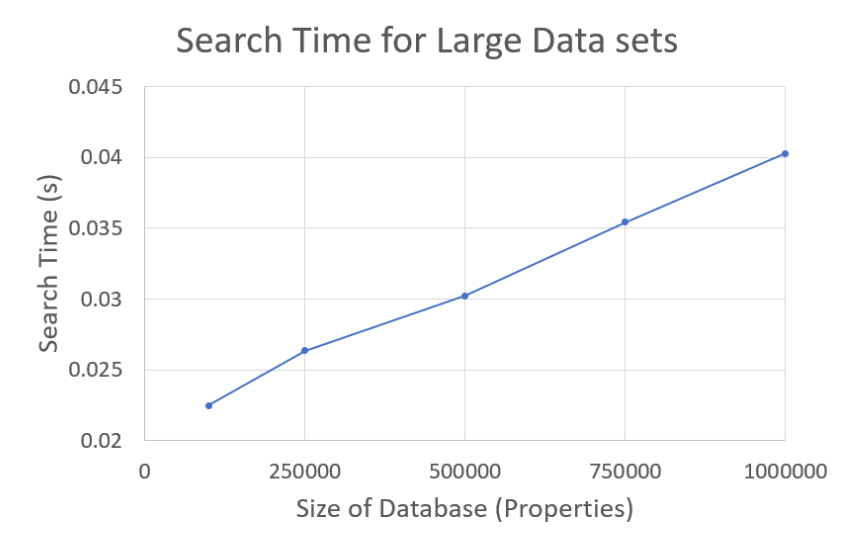
\includegraphics[width=\linewidth]{assets/performancetest.png}
  \caption{Performance of large data sets}
  \label{fig:performancetest}
\end{figure}

As can be seen in Figure \ref{fig:performancetest}, the search time for large
property data sets appears to increase linearly. For a database with one million
properties, it takes only 0.04 seconds to complete the search. This can be mostly
be attributed to the initial filter, which drastically cuts down search time.

\newpage
\subsection{Real Time Communication}\label{realtime}

The real-time communication powering platform features such as notifications,
instant messaging, and bidding events, is provided through the use of web
sockets. WebSockets allow for bi-directional messages to be instantly
communicated with minimal overhead \parencite{websocket}. While Django doesn't
provide support for WebSockets, support can be provided through a third-party
extension for Django called Django Channels.

\subsubsection{MSocket Library \& Django Channels}

Django Channels does not provide native support for multiplex sockets. When
a client application begins listening to an event it must dedicate an entire
socket. Consequently, a client may have multiple sockets open to send and
receive messages for individual events despite the fact that the traffic could
be sent over a single socket. A server only has a limited number of sockets
available so this reduces the scalability by a significant factor. Multiplex
sockets are sockets that are used to transmit information of different classes
that are then filtered by the receiver and forwarded to the correct recipient
(See Figure \ref{fig:msocket}).

To ensure that \emph{localhost} was scalable, support for multiplex sockets
was provided with a custom client-side JavaScript library and custom Django
class.
\begin{figure}[!h]
  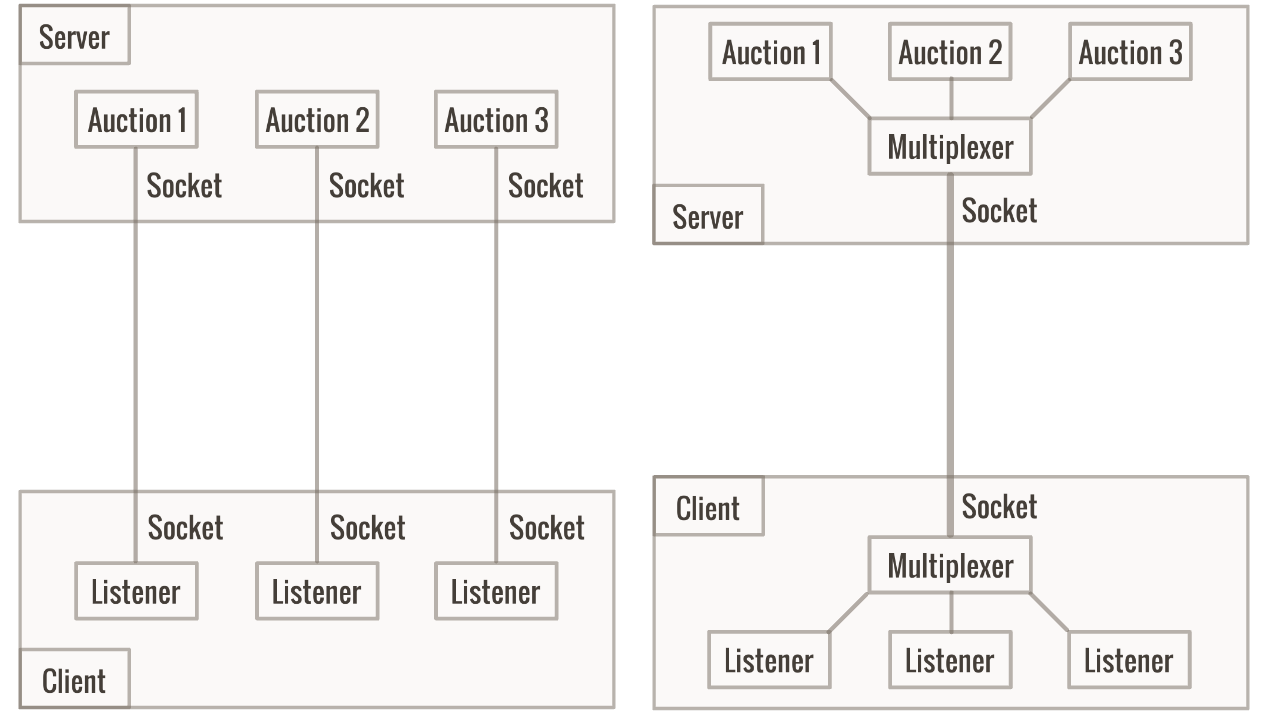
\includegraphics[width=\linewidth]{assets/msocket.png}
  \caption{Comparison between regular sockets and multiplexed sockets}
  \label{fig:msocket}
\end{figure}
The client-side library, called \emph{msocket.js}, is a cooperative multiplex
socket libary. This means that for the socket multiplexing to work, the client
and server must adopt a common protocol of communication. The protocol used
in \emph{localhost} is provided below in the form of a JSON file.
\begin{lstlisting}
{
  type: ,
  data: {

  }
}
\end{lstlisting}

The type allows the multiplexer to determine how to handle the message, and
the data is the payload for the
message. In the case of real-time bidding, the payload would contain details
allowing the handler to determine which property item the bid is for, and how
much the bid is.

\emph{msocket.js} is designed from scratch to provide a simple and abstracted
interface to hide away the details and complexity behind WebSockets. A client
can submit handlers to execute for different types (shown below) and they will
automatically execute as messages of that type arrive.
\begin{lstlisting}
  /**
   * @brief Registers a handler for a message type
   *
   * @param type    The type of message the handler should apply to
   * @param handler The handler to execute on message recieve
   *                Should take the data as an argument
   *                See JSON specification
   *
   * @return On success, @c true
   * @return On failure, @c false when a handler is already set for the type
   * */
  register_handler(type, handler);
\end{lstlisting}

Server-side, the Django Channels socket consumer class was modified to maintain
a record of each of the events the socket is subscribed to and whenever a
message is broadcasted for one of these events the consumer transmits it to
the client with the appropriate class identifier.

\subsection{Event Scheduling}
When an auction session ends, tasks need to be performed in order to complete
the bidding process. There are also several places where scheduled/delayed tasks
are needed in the application.

Property items are said to be ``available'' if the \emph{available} option is
turned on by user (it is ``on'' by default when created) and there are no bids
in all the previous auction sessions in the same day. When the local time
reaches the end time of the session, the system have to check whether there are
bids in the session and create a booking for the winner. Property items that has
been booked out has to be marked as ``unavailable'' so that it does not come up
in the search results. Furthermore, property item has to be re-listed (marked
as ``available'') at 12 noon every day.

\subsubsection{Django Signals}
Signals are dispatched in Django when a certain action is performed within the
framework. It helps decoupled applications to get notified when the actions are
taken placed~\parencite{django-signals}. Django provides a set of built-in signals
that allows us to combine it with Celery to perform certain tasks when signals
are dispatched. A list of signals we used in the project are:

\begin{itemize}
  \item \texttt{django.db.models.signals.m2m\_changed}
  \item \texttt{django.db.models.signals.pre\_save}
\end{itemize}

\subsubsection{Celery Beat}
Celery beat is a scheduler in Celery that kicks off tasks at regular intervals,
that are then executed by available worker nodes in the cluster~\parencite{celery-beat}.
The worker works asynchronously to start task execution and store results in
a Redis instance.

By default, beat uses \texttt{PersistentScheduler} that keeps track of the last
run in a local shelve\footnote{a persistent, dictionary-like object} database
file. But that is not necessary since we already have a PostgreSQL database
active in the back-end. So we instead use an extension
django-celery-beat~\ref{sec:dep-celery-beat} that allows us to store tasks in
the Django database through a \texttt{DatabaseScheduler}. The extension also
provides an admin interface so that tasks could be managed by the administrator.

\paragraph{Periodic Task}
\texttt{PeriodicTask} is a Django model provided by
django-celery-beat~\ref{sec:dep-celery-beat} that simulates how Celery tasks are
represented in the database. We use this in conjunction with
\texttt{DatabaseScheduler} to provide background services in the Django
framework.

\subsubsection{Combining both signals and Celery beat}
There are two tasks to be completed in the background:
\begin{enumerate}
  \item check if anyone bid on a property item; if there is, a booking is added
    to the winner's account, and bids associated with the property item are
    removed. Property item is marked as ``unavailable'' as well. Otherwise we do
    nothing about that property item.
  \item enable bidding for all property items at 12 noon
\end{enumerate}
As such, we define two tasks in Celery accordingly: \texttt{cleanup\_bids} and
\texttt{enable\_bids}. Whenever an auction session is added to a property item
(\texttt{m2m\_changed}), we add a \texttt{PeriodicTask} to the database that
executes \texttt{cleanup\_bids}. A \texttt{PeriodicTask} that executes
\texttt{enable\_bids} is added when a property item is
saved (\texttt{pre\_save}). When celery is launched, the scheduler will pick up
the tasks and triggers tasks execution when time reaches.
